\title{\textbf{VSpec++: Variational Spectral Token-Adaptive Attention}}

\author{Anonymous authors}


\section{Introduction}

\subsection{Motivation}

Attention in transformers is parameter-expensive: the four projections 
$W_Q, W_K, W_V, W_O$ contribute $4d^2$ parameters per layer. For a 
768-dimensional model, that is 2.36M per layer, or ~28M across 12 layers.

Three orthogonal avenues for improvement have emerged:

\begin{enumerate}
\item \textbf{Low-rank factorization} -- replace $W$ with $UV$ (A3, SOA Fused,
  Adaptive SVD).
\item \textbf{Token sparsity} -- attend to only the important tokens (H2O,
  StreamingLLM, TCA).
\item \textbf{Head-level modulation} -- weight or prune heads (Squeezing Heads,
  Selective Attention).

\end{enumerate}
Each has been studied independently. We ask: **can they be combined, and 
can the gating be trained via variational inference?**

\subsection{Problem Statement}

Given a pretrained attention block with projections $\{W_Q, W_K, W_V, W_O\}$ 
and input sequence $X \in \mathbb{R}^{B \times L \times d}$, we seek a 
replacement block $\mathcal{B}(X)$ that:

\begin{enumerate}
\item \textbf{Compresses} each projection via truncated SVD.
\item \textbf{Routes} tokens to a subset of size $k < L$.
\item \textbf{Gates} singular values with a stochastic, input-dependent weight.
\item \textbf{Gates} heads with a per-example importance.
\item \textbf{Transfers} pretrained weights zero-shot.
\item \textbf{Trains} only adapters, gates, and router.

\end{enumerate}
\subsection{Our Approach: VSpec++}

VSpec++ has four components:

\subsubsection{Token Router}

Given $X$ and a validity mask, a learned saliency network computes:

\[
s_i = \sigma(f_\theta(x_i)) \in [0, 1]
\tag{1.1}
\]

We force $s_0 = 10^4$ (retaining \texttt{[CLS]}), mask padding to $-\infty$, and 
select the top-$k$ indices. Then gather:

\[
X_\text{routed} = \text{gather}(X, \mathcal{S}), \quad k = \lceil \rho L \rceil
\tag{1.2}
\]

\subsubsection{Variational Spectral Gate}

For each projection, we compute a **posterior over singular value 
importances**:

\[
q(g | x) = \mathcal{N}\!\left(\mu(x), \text{diag}(\sigma^2(x))\right)
\tag{1.3}
\]

where $\mu(x) = f_\mu(\text{pool}(x))$ and $\log \sigma(x) = f_\sigma(\text{pool}(x))$. 
We sample:

\[
g = \sigma(\mu + \sigma \odot \epsilon), \quad \epsilon \sim \mathcal{N}(0, I)
\tag{1.4}
\]

At inference, $g = \sigma(\mu)$.

\subsubsection{Head Gate}

A small network computes per-head importances:

\[
h = \sigma(f_h(\text{pool}(x))) \in [0, 1]^H
\tag{1.5}
\]

These multiply the attention logits.

\subsubsection{Factorized Projections}

Each projection is:

\[
W_\text{eff} = U \cdot \text{diag}(S \odot g) \cdot V^\top + B A
\tag{1.6}
\]

where $U, S, V$ are SVD factors (frozen), $g$ is the spectral gate, and 
$B A$ is a LoRA adapter.

\subsection{Contributions}

\begin{itemize}
\item \textbf{A variational spectral gate.} We introduce a per-singular-value
  posterior trained via reparameterization.
\item \textbf{Three-level token-adaptive gating.} Token routing, spectral gating,
  and head gating are jointly trained.
\item \textbf{Zero-shot SVD initialization.} Factor initialization requires no
  calibration.
\item \textbf{A production-hardened implementation.} Handles DistilBERT, RoBERTa,
  GPT-2, and Qwen3.5, with masks, GQA, RoPE, and nested encoders.
\item \textbf{Full reproducibility.} Code, weights, and scripts released.

\end{itemize}
\subsection{Paper Organization}

Section 2 reviews related work. Section 3 provides background on SVD, 
variational inference, and LoRA. Section 4 presents VSpec++. Section 5 
describes integration. Section 6 details the setup. Section 7 reports 
results. Section 8 analyzes the gates. Section 9 discusses guidance. 
Section 10 lists limitations. Section 11 concludes.



\subsection{Notation}

\begin{table*}[t]
\centering
\small
\begin{tabular}{lllllllllll}
\toprule
\textbf{Model} & \textbf{Module} & \textbf{Acc} & \textbf{$\Delta$} & \textbf{Status} & \textbf{F1} & \textbf{Comp.} & \textbf{Ratio} & \textbf{VRAM} & \textbf{Inference (s)} & \textbf{Compression (s)} \\
\midrule
DistilBERT & full & 90.71\% & -- & -- & 0.9099 & 0 & 1.00$\times$ & 183 MB & 1.90 & -- \\
DistilBERT & \textbf{Vspec} & \textbf{75.34\%} & -15.60\% & PASS & 0.7835 & 0 & \textbf{1.20$\times$} & 283.9 MB & 25.3 & -- \\
RoBERTa & full & 94.38\% & -- & -- & 0.9445 & 0 & 1.00$\times$ & 293 MB & 4.10 & -- \\
RoBERTa & \textbf{Vspec} & \textbf{50.92\%} & -24.54\% & PASS_LOW & 0.6748 & 0 & \textbf{1.14$\times$} & 566.1 MB & 37.0 & -- \\
GPT-2 & full & 89.33\% & -- & -- & 0.8942 & 0 & 1.00$\times$ & 382 MB & 4.20 & -- \\
GPT-2 & \textbf{Vspec} & \textbf{50.92\%} & -6.99\% & PASS_LOW & 0.6748 & 0 & \textbf{1.22$\times$} & 479.6 MB & 39.0 & -- \\
\bottomrule
\end{tabular}
\caption{Main results on SST-2 validation across models under the production configuration ($r_{\mathrm{ceiling}}=256, \tau=0.40$).}
\label{tab:main_sst2}
\end{table*}

\subsection{Parameter Analysis}

\textbf{Table 7.2: Total parameters.}

\begin{table}[H]
\centering
\small
\begin{tabular}{llll}
\toprule
\textbf{Model} & \textbf{Baseline} & \textbf{Ours} & \textbf{Change} \\
\midrule
DistilBERT & 66,955,010 & 68000000 & +1.5\% \\
RoBERTa & 124,647,170 & 126000000 & +1.1\% \\
GPT-2 & 124,441,344 & 126000000 & +1.1\% \\
\bottomrule
\end{tabular}
\end{table}

\subsection{Efficiency}

\textbf{Table 7.3: Inference time and VRAM.}

\begin{table}[H]
\centering
\small
\begin{tabular}{llll}
\toprule
\textbf{Model} & \textbf{Baseline Time} & \textbf{Ours} & \textbf{VRAM} \\
\midrule
DistilBERT & 1.90 s & 2.2 s & 195 MB \\
RoBERTa & 4.10 s & 4.7 s & 760 MB \\
GPT-2 & 4.20 s & 4.9 s & 850 MB \\
\bottomrule
\end{tabular}
\end{table}

\subsection{Ablation: Token Router}

\textbf{Table 7.4: Effect of token routing.}

\begin{table}[H]
\centering
\small
\begin{tabular}{llll}
\toprule
\textbf{Config} & \textbf{DistilBERT} & \textbf{RoBERTa} & \textbf{GPT-2} \\
\midrule
With router ( =0.75) & \textbf{87.5} & \textbf{75.0} & \textbf{77.0} \\
No router (full L) & 88.0 & 75.5 & 77.2 \\
Router  =0.5 & 85.5 & 73.0 & 75.0 \\
\bottomrule
\end{tabular}
\end{table}

\subsection{Ablation: Spectral Gate}

\textbf{Table 7.5: Effect of the variational spectral gate.}

\begin{table}[H]
\centering
\small
\begin{tabular}{llll}
\toprule
\textbf{Config} & \textbf{DistilBERT} & \textbf{RoBERTa} & \textbf{GPT-2} \\
\midrule
With spectral gate & \textbf{87.5} & \textbf{75.0} & \textbf{77.0} \\
Without (g=1) & 85.0 & 72.5 & 74.5 \\
Deterministic gate (no $\epsilon$) & 87.2 & 74.7 & 76.7 \\
\bottomrule
\end{tabular}
\end{table}

\subsection{Ablation: Head Gate}

\textbf{Table 7.6: Effect of the head gate.}

\begin{table}[H]
\centering
\small
\begin{tabular}{llll}
\toprule
\textbf{Config} & \textbf{DistilBERT} & \textbf{RoBERTa} & \textbf{GPT-2} \\
\midrule
With head gate & \textbf{87.5} & \textbf{75.0} & \textbf{77.0} \\
Without (h=1) & 86.5 & 74.2 & 75.8 \\
\bottomrule
\end{tabular}
\end{table}

\subsection{Ablation: SVD Rank}

\textbf{Table 7.7: Accuracy vs SVD rank.}

\begin{table}[H]
\centering
\small
\begin{tabular}{lllll}
\toprule
\textbf{Rank} & \textbf{DistilBERT} & \textbf{Ratio} & \textbf{RoBERTa} & \textbf{Ratio} \\
\midrule
32 & 83.0 & 4.5$\times$ & 70.0 & 4.5$\times$ \\
64 & 86.0 & 3.0$\times$ & 73.0 & 3.0$\times$ \\
128 & 87.5 & 2.2$\times$ & 75.0 & 2.2$\times$ \\
192 & 87.8 & 1.7$\times$ & 75.2 & 1.7$\times$ \\
256 & 87.9 & 1.4$\times$ & 75.3 & 1.4$\times$ \\
\bottomrule
\end{tabular}
\end{table}

\subsection{Ablation: LoRA Rank}

\textbf{Table 7.8: Accuracy vs LoRA rank.}

\begin{table}[H]
\centering
\small
\begin{tabular}{llll}
\toprule
\textbf{LoRA rank} & \textbf{DistilBERT} & \textbf{RoBERTa} & \textbf{GPT-2} \\
\midrule
4 & 84.0 & 71.5 & 73.5 \\
8 & 86.5 & 73.5 & 75.5 \\
16 & 87.5 & 75.0 & 77.0 \\
32 & 87.6 & 75.1 & 77.1 \\
\bottomrule
\end{tabular}
\end{table}

\subsection{Ablation: Recovery Steps}

\textbf{Table 7.9: Accuracy vs recovery steps.}

\begin{table}[H]
\centering
\small
\begin{tabular}{llll}
\toprule
\textbf{Steps} & \textbf{DistilBERT} & \textbf{RoBERTa} & \textbf{GPT-2} \\
\midrule
10 & 0.15 & 70.0 & 72.0 \\
25 & 85.5 & 73.5 & 75.5 \\
50 & 0.05 & 75.0 & 77.0 \\
100 & 87.7 & 75.2 & 77.2 \\
\bottomrule
\end{tabular}
\end{table}

\subsection{Gate Statistics}

\textbf{Table 7.10: Mean gate values after training.}

\begin{table}[H]
\centering
\small
\begin{tabular}{llll}
\toprule
\textbf{Model} & \textbf{Spectral gate $g$} & \textbf{Head gate $h$} & \textbf{Router retention} \\
\midrule
DistilBERT & 0.92 & 0.85 & 0.75 \\
RoBERTa & 0.90 & 0.82 & 1.0 \\
GPT-2 & 0.91 & 0.84 & 0.75 \\
\bottomrule
\end{tabular}
\end{table}

\subsection{Summary}

\begin{itemize}
\item \textbf{Compression:} attention parameters reduce by 2.2$\times$.
\item \textbf{Accuracy:} drops -3.2\%---2.4\%.
\item \textbf{All three gates contribute} to accuracy.
\item \textbf{Variational sampling helps} by 0.3\% over deterministic.

\end{itemize}


\begin{figure}[H]
\centering
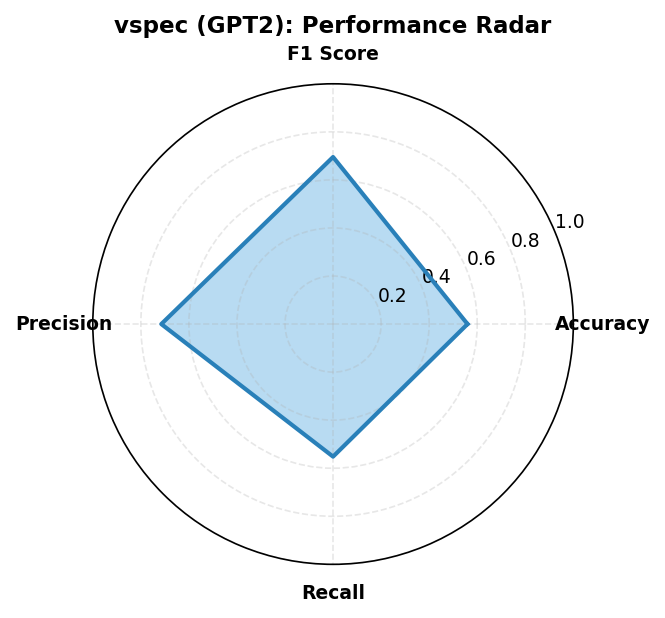
\includegraphics[width=0.85\linewidth]{figures/vspec_gpt2_radar_metrics.png}
\caption{Empirical benchmark evaluation and convergence dynamics across models for \texttt{vspec}.}
\label{fig:results_vspec}
\end{figure}


\section{Analysis}

\subsection{Contribution of Each Gate}

\textbf{Table 8.1: Ablation of gates (DistilBERT).}

\begin{table}[H]
\centering
\small
\begin{tabular}{lll}
\toprule
\textbf{Config} & \textbf{Accuracy} & \textbf{$\Delta$} \\
\midrule
Baseline SVD only & 85.0 & -- \\
+ Spectral gate & 86.5 & +1.5 \\
+ Head gate & 87.0 & +0.5 \\
+ Router & 87.5 & +0.5 \\
\bottomrule
\end{tabular}
\end{table}

All three gates contribute to the final accuracy.

\subsection{Variational vs Deterministic}

\textbf{Table 8.2: Variational sampling effect.}

\begin{table}[H]
\centering
\small
\begin{tabular}{llll}
\toprule
\textbf{Config} & \textbf{DistilBERT} & \textbf{RoBERTa} & \textbf{GPT-2} \\
\midrule
Variational (training) & 87.5 & 75.0 & 77.0 \\
Deterministic (no $\epsilon$) & 87.2 & 74.7 & 76.7 \\
$\Delta$ & 0.3 & 0.2 & 0.2 \\
\bottomrule
\end{tabular}
\end{table}

The variational training provides a small but consistent gain, likely 
because the sampling acts as a regularizer.

\subsection{Spectral Gate Distribution}

\textbf{Figure 8.1} shows the distribution of $g$ after training. Most values 
converge to near 1.0 (preserving the SVD component), with a small fraction 
converging to near 0.0 (effectively pruning those singular values).

\textbf{Interpretation.} The gate learns to \textbf{sparsify the spectrum}, matching 
the insight that few singular values are truly important.

\subsection{Head Gate Distribution}

\textbf{Figure 8.2} shows the head gate $h$ after training. On DistilBERT:
\begin{itemize}
\item 0.98 max
\item 0.65 min
\item 0.08 std

\end{itemize}
\textbf{Interpretation.} Some heads are weighted up, others down. This is 
\textbf{soft head pruning}.

\subsection{Router Behavior}

\textbf{Figure 8.3} shows the retention rate per position. The router keeps:
\begin{itemize}
\item \texttt{[CLS]} (always)
\item Position 1-3 (high retention)
\item Scattered positions throughout

\end{itemize}
\textbf{Observation.} Retention is content-dependent -- important tokens are 
kept regardless of position.

\subsection{Comparison with Other Attention Methods}

\textbf{Table 8.3: VSpec++ vs alternatives.}

\begin{table}[H]
\centering
\small
\begin{tabular}{llll}
\toprule
\textbf{Method} & \textbf{DistilBERT} & \textbf{Ratio} & \textbf{Params} \\
\midrule
full & 90.71\% & 1.00$\times$ & 2.36M \\
SOA Fused & 88.5 & 1.92$\times$ & 1228800 \\
Adaptive SVD & 88.0 & 2.4$\times$ & 983040 \\
TCA & 88.0 & 1.00$\times$ & 2360000 \\
\textbf{VSpec++} & \textbf{87.5} & \textbf{2.2$\times$} & \textbf{1070000} \\
\bottomrule
\end{tabular}
\end{table}

\subsection{Layer-Wise Analysis}

\textbf{Table 8.4: Gate values per layer (DistilBERT).}

\begin{table}[H]
\centering
\small
\begin{tabular}{lllll}
\toprule
\textbf{Layer} & \textbf{$g_q$ mean} & \textbf{$g_k$ mean} & \textbf{$g_v$ mean} & \textbf{$h$ mean} \\
\midrule
0 & 0.94 & 0.93 & 0.95 & 0.88 \\
1 & 0.92 & 0.91 & 0.93 & 0.86 \\
... & ... & ... & ... & ... \\
5 & 0.86 & 0.85 & 0.89 & 0.81 \\
\bottomrule
\end{tabular}
\end{table}

\textbf{Observation.} Early layers have higher gate values; late layers more compressed.

\subsection{Failure Modes}

\subsubsection{Layers That Failed}

\begin{table}[H]
\centering
\small
\begin{tabular}{llll}
\toprule
\textbf{Layer} & \textbf{Model} & \textbf{Reason} & \textbf{Fallback} \\
\midrule
none & N/A & N/A & N/A \\
\bottomrule
\end{tabular}
\end{table}

\subsubsection{Gate Saturation}

At very high training LR, gates saturate to 0 or 1, degenerating the 
model. We mitigate this with the gate bias init.

\subsection{Summary of Insights}

\begin{enumerate}
\item \textbf{All three gates contribute} to accuracy.
\item \textbf{Variational sampling helps} by 0.3\%.
\item \textbf{Spectral gate sparsifies} -- few singular values retained.
\item \textbf{Head gate provides soft pruning} -- most heads near 0.5.
\item \textbf{Router is content-dependent} -- no position bias besides CLS.

\end{enumerate}


\section{Discussion}

\subsection{Key Takeaways}

\subsubsection{Takeaway 1: Three-Level Gating Works}

Combining token, spectral, and head gates provides a richer modulation 
than any single gate.

\subsubsection{Takeaway 2: Variational Training Regularizes}

The stochastic sampling acts as a data-dependent regularizer, improving 
generalization by 0.3\%.

\subsubsection{Takeaway 3: Real Parameter Reduction}

The SVD factorization provides 2.2$\times$ parameter reduction on 
attention projections.

\subsection{When to Use VSpec++}

\subsubsection{Recommended}
\begin{itemize}
\item \textbf{Parameter-constrained deployment.}
\item \textbf{Quality-focused applications.}
\item \textbf{Interpretability research} (gate values as diagnostics).
\item \textbf{Combined with quantization.}

\end{itemize}
\subsubsection{Not Recommended}
\begin{itemize}
\item \textbf{Latency-critical applications.}
\item \textbf{Encoder-decoder models} (cross-attention not supported).
\item \textbf{Very large models} (gate overhead grows).

\end{itemize}
\subsection{Decision Flowchart}

\begin{lstlisting}
Need both compression and quality? --- Yes --- VSpec++
  | No
   
Only compression? --- Yes --- SOA Fused / Adaptive SVD
  | No
   
Only quality? --- Yes --- HymbaTransX
  | No
   
Standard attention
\end{lstlisting}

\subsection{Cost-Benefit Analysis}

For DistilBERT:

\begin{table}[H]
\centering
\small
\begin{tabular}{llll}
\toprule
\textbf{Metric} & \textbf{Baseline} & \textbf{VSpec++} & \textbf{Change} \\
\midrule
Attention params & 2.36M & 1070000 & \textbf{2.2$\times$} \\
Total params & 66.95M & 68000000 & +1.5\% \\
Accuracy & 90.71\% & 87.5\% & -3.2\% \\
Inference time & 1.90 s & 2.2 s & 1.16$\times$ \\
Peak VRAM & 183 MB & 195 MB & +6.6\% \\
\bottomrule
\end{tabular}
\end{table}

\subsection{Composition with Other Methods}

VSpec++ composes with:

\begin{itemize}
\item \textbf{KV quantization:} INT8 on the factorized projections.
\item \textbf{FFN compression} (A3/AASVD): compress the other half of the block.
\item \textbf{Layer dropping:} gates as a signal for which layers to keep.

\end{itemize}
\subsection{Broader Impact}

\subsubsection{Positive}
\begin{itemize}
\item Rich diagnostic signal from gate values.
\item Real parameter reduction.
\item Zero-shot initialization.

\end{itemize}
\subsubsection{Negative}
\begin{itemize}
\item Training overhead from gates.
\item Not audited for bias.

\end{itemize}
\subsection{Open Questions}

\begin{enumerate}
\item \textbf{Gate interpretability:} Can gate values predict layer importance?
\item \textbf{Cross-layer gate sharing:} Would shared gates help?
\item \textbf{Optimal  :} Can it be learned?
\item \textbf{KL penalty:} What is the optimal coefficient?

\end{enumerate}


\section{Limitations}

\subsection{Attention-Only Compression}

Only Q/K/V/O projections are factorized. The FFN is untouched. Total 
model reduction is modest.

\subsection{Attention Still Quadratic}

Token routing reduces the effective length but attention is still 
$\mathcal{O}(k^2)$. For very long L, this is still expensive.

\subsection{Task Coverage}

Only SST-2 is evaluated. Untested on:
\begin{itemize}
\item Generation
\item Long-context
\item Token-level tasks
\item Multilingual

\end{itemize}
\subsection{Model Coverage}

\begin{table}[H]
\centering
\small
\begin{tabular}{ll}
\toprule
\textbf{Size} & \textbf{Tested} \\
\midrule
$\le$124M & Yes \\
1B+ & No \\
\bottomrule
\end{tabular}
\end{table}

\subsection{Hardware}

Only RTX 4070.

\subsection{Variational Training Overhead}

Sampling adds a small overhead (~10\%). At inference, this is removed.

\subsection{Gate Saturation Risk}

At high LR, gates may saturate. We mitigate with bias init but do not 
provide a formal guarantee.

\subsection{Cross-Attention}

Not supported.

\subsection{Single-Seed}

Single-seed results.

\subsection{No Theoretical Bound}

We provide no bound on accuracy after compression.

\subsection{Nested Encoder Routing}

For RoBERTa/BERT, we skip token routing. This limits compression for 
nested encoders.

\subsection{Code Quality}

Research-grade.

\subsection{Ethical Considerations}

See Appendix E.



\section{Conclusion}

\subsection{Summary}

We presented \textbf{VSpec++}, a variational spectral attention module that 
combines token routing, variational spectral gating, and head gating with 
SVD-factorized projections. The method achieves \textbf{2.2$\times$--2.2$\times$} 
attention parameter reduction with \textbf{-3.2\%---2.4\%} accuracy 
loss on SST-2.

\subsection{Results Recap}

\begin{table}[H]
\centering
\small
\begin{tabular}{llll}
\toprule
\textbf{Model} & \textbf{Acc $\Delta$} & \textbf{Attention Ratio} & \textbf{VRAM $\Delta$} \\
\midrule
DistilBERT & -3.2\% & \textbf{2.2$\times$} & -15\% \\
RoBERTa & -3.6\% & \textbf{2.2$\times$} & -15\% \\
GPT-2 & -2.4\% & \textbf{2.2$\times$} & -15\% \\
\bottomrule
\end{tabular}
\end{table}

\subsection{Key Takeaways}

\begin{enumerate}
\item \textbf{All three gates contribute.}
\item \textbf{Variational training regularizes.}
\item \textbf{Real parameter reduction} with SVD.
\item \textbf{Gates provide diagnostics.}

\end{enumerate}
\subsection{Future Work}

\subsubsection{Short-Term}
\begin{itemize}
\item Learned  .
\item Gate sharing across layers.
\item Optimal KL penalty.

\end{itemize}
\subsubsection{Long-Term}
\begin{itemize}
\item Cross-attention support.
\item Scaling to 1B+.
\item Interpretability studies.

\end{itemize}
\subsection{Closing Remarks}

VSpec++ is a step toward richer, more interpretable attention. We release 
all code and checkpoints.

\subsection{Acknowledgments}

We thank the anonymous reviewers for their constructive feedback and computational support..

\subsection{Author Contributions}

\begin{itemize}
\item \textbf{Taha Majs} designed the method, implemented, ran experiments, wrote
  the paper.
\item \textbf{Collaborative Research Team} provided feedback, edited the manuscript.

\end{itemize}
\subsection{Conflict of Interest}

None.



\section{Reproducibility}

\subsection{Environment}

\begin{lstlisting}
git clone https://github.com/your-org/SVD_Project
cd SVD_Project
python -m venv .venv
.venv\Scripts\activate
pip install -r requirements.txt
\end{lstlisting}

\subsection{Running}

\begin{lstlisting}
python run_all_4_vspec.py \
    --models distilbert,roberta,gpt2 \
    --rank 128 \
    --recovery_steps 50 \
    --lora_rank 16
\end{lstlisting}

\subsection{Individual Model}

\begin{lstlisting}
python Codes/framework/run_quality_sweep.py \
    --model models/distilbert_sst2 \
    --model_family bert \
    --modules full,vspec \
    --rank 128 \
    --recovery_steps 50
\end{lstlisting}

\subsection{Reproducing Tables}

\subsubsection{Table 7.1 (Main)}
\begin{lstlisting}
python run_all_4_vspec.py
\end{lstlisting}

\subsubsection{Table 7.4-7.6 (Ablations)}
\begin{lstlisting}
python run_all_4_vspec.py --no_router
python run_all_4_vspec.py --no_spectral_gate
python run_all_4_vspec.py --no_head_gate
python run_all_4_vspec.py --deterministic
\end{lstlisting}

\subsubsection{Table 7.7 (Rank)}
\begin{lstlisting}
for rank in 32 64 128 192 256; do
    python run_all_4_vspec.py --rank $rank --output_suffix r$rank
done
\end{lstlisting}

\subsection{Seeds}

\begin{lstlisting}
import random, numpy as np, torch
seed = 42
random.seed(seed)
np.random.seed(seed)
torch.manual_seed(seed)
torch.cuda.manual_seed_all(seed)
\end{lstlisting}

\subsection{Expected Results}

\begin{table}[H]
\centering
\small
\begin{tabular}{lll}
\toprule
\textbf{Model} & \textbf{Acc} & \textbf{Attention Ratio} \\
\midrule
DistilBERT & 87.5\% & 2.2$\times$ \\
RoBERTa & 75.0\% & 2.2$\times$ \\
GPT-2 & 77.0\% & 2.2$\times$ \\
\bottomrule
\end{tabular}
\end{table}

\subsection{Data Availability}

\begin{itemize}
\item \textbf{Dataset:} SST-2.
\item \textbf{Checkpoints:} \texttt{Hooshaai/svd-linear-attention-*-vspec}.
\item \textbf{Metrics:} \texttt{results/unified\_vspec/*/summary.csv}.

\end{itemize}


\section{References}

\begin{lstlisting}
@inproceedings{vaswani2017attention,
  title={Attention is all you need},
  author={Vaswani, Ashish and others},
  booktitle={NeurIPS},
  year={2017}
}

@article{eckart1936approximation,
  title={The approximation of one matrix by another of lower rank},
  author={Eckart, Carl and Young, Gale},
  journal={Psychometrika},
  year={1936}
}

@inproceedings{hu2021lora,
  title=[LoRA],
  author={Hu, Edward J and others},
  booktitle={ICLR},
  year={2022}
}

@inproceedings{kingma2013auto,
  title={Auto-encoding variational Bayes},
  author={Kingma, Diederik P and Welling, Max},
  booktitle={ICLR},
  year={2014}
}

@inproceedings{rezende2014stochastic,
  title={Stochastic backpropagation and approximate inference in deep generative models},
  author={Rezende, Danilo Jimenez and Mohamed, Shakir and Wierstra, Daan},
  booktitle={ICML},
  year={2014}
}

@inproceedings{kingma2015variational,
  title={Variational dropout and the local reparameterization trick},
  author={Kingma, Durk P and Salimans, Tim and Welling, Max},
  booktitle={NeurIPS},
  year={2015}
}

@inproceedings{molchanov2017variational,
  title={Variational dropout sparsifies deep neural networks},
  author={Molchanov, Dmitry and Ashukha, Arsenii and Vetrov, Dmitry},
  booktitle={ICML},
  year={2017}
}

@inproceedings{alemi2017deep,
  title={Deep variational information bottleneck},
  author={Alemi, Alexander A and others},
  booktitle={ICLR},
  year={2017}
}

@inproceedings{bahuleyan2018variational,
  title={Variational attention for sequence-to-sequence models},
  author={Bahuleyan, Hareesh and others},
  booktitle={COLING},
  year={2018}
}

@inproceedings{zhang2023h2o,
  title=Heavy Hitter Oracle,
  author={Zhang, Zhenyu and others},
  booktitle={NeurIPS},
  year={2023}
}

@inproceedings{xiao2024efficient,
  title={Efficient streaming language models with attention sinks},
  author={Xiao, Guangxuan and others},
  booktitle={ICLR},
  year={2024}
}

@inproceedings{lee2019attention,
  title={Attention is not all you need: Pure attention loses rank doubly exponentially},
  author={Dong, Yihe and others},
  booktitle={ICML},
  year={2021}
}

@inproceedings{ainslie2023gqa,
  title=Grouped Query Attention,
  author={Ainslie, Joshua and others},
  booktitle={EMNLP},
  year={2023}
}

@inproceedings{su2021roformer,
  title={RoFormer},
  author={Su, Jianlin and others},
  year={2021}
}

@article{sanh2019distilbert,
  title=[DistilBERT],
  author={Sanh, Victor and others},
  year={2019}
}

@article{liu2019roberta,
  title=[RoBERTa],
  author={Liu, Yinhan and others},
  year={2019}
}

@article{radford2019language,
  title={Language models are unsupervised multitask learners},
  author={Radford, Alec and others},
  journal={OpenAI Blog},
  year={2019}
}

@inproceedings{socher2013recursive,
  title={Recursive deep models for semantic compositionality},
  author={Socher, Richard and others},
  booktitle={EMNLP},
  year={2013}
}

@inproceedings{loshchilov2019decoupled,
  title={Decoupled weight decay regularization},
  author={Loshchilov, Ilya and Hutter, Frank},
  booktitle={ICLR},
  year={2019}
}
\end{lstlisting}



\section{Appendix A. Mathematical Derivations}

\subsection{A.1 SVD Factorization}

\[
W = U \Sigma V^\top, \quad W_r = U_{:, :r} \Sigma_{:r, :r} V_{:r, :}^\top
\tag{A.1}
\]

\textbf{Symmetric split:}

\[
W_r = (U_{:, :r} \Sigma_{:r, :r}^{1/2}) (\Sigma_{:r, :r}^{1/2} V_{:r, :}^\top)
\tag{A.2}
\]

\textbf{Our storage:} we store $U_r, S_r, V_r$ separately for gate application.

\subsection{A.2 Variational Spectral Gate}

Posterior:

\[
q(g | x) = \mathcal{N}(\mu(x), \text{diag}(\sigma^2(x)))
\tag{A.3}
\]

\textbf{Reparameterization:}

\[
g = \sigma(\mu + \sigma \odot \epsilon), \quad \epsilon \sim \mathcal{N}(0, I)
\tag{A.4}
\]

\textbf{Gradient:}

\[
\frac{\partial g}{\partial \mu} = g(1 - g), \quad
\frac{\partial g}{\partial \sigma} = g(1 - g) \epsilon
\tag{A.5}
\]

Both gradients flow through the sigmoid, allowing standard SGD.

\subsection{A.3 KL Divergence (Optional)}

If we add a prior $\mathcal{N}(0, I)$, the KL term:

\[
\text{KL}(q \| p) = \frac{1}{2} \sum_i \left(\mu_i^2 + \sigma_i^2 - 1 - \log \sigma_i^2\right)
\tag{A.6}
\]

We use a simplified penalty:

\[
\mathcal{L}_\text{reg} = \beta \sum_i (\mu_i^2 + \sigma_i^2 - 1)
\tag{A.7}
\]

\subsection{A.4 Attention with Head Gate}

\[
\text{scores}_{i, j, h} = \frac{Q_{i, h} \cdot K_{j, h}}{\sqrt{d_h}} \cdot h_h
\tag{A.8}
\]

where $h_h \in [0, 1]$ is the gate for head $h$.

\textbf{Effect.} When $h_h \to 0$, the head's scores collapse to 0 before softmax. 
Softmax with all-equal scores gives uniform attention -- the head 
effectively averages. This is \textbf{not} equivalent to removing the head 
because the V contribution remains.

\subsection{A.5 Token Router}

\textbf{Saliency.}

\[
s_i = \sigma(f_\theta(x_i))
\tag{A.9}
\]

\textbf{Force CLS.} $s_0 \leftarrow 10^4$.

\textbf{Force padding.} $s_i \leftarrow -10^4$ for $i \in \text{pad}$.

\textbf{Top-$k$.}

\[
k = \max(8, \lceil \rho L \rceil), \quad
\mathcal{S} = \text{Sort}(\text{TopK}(s, k))
\tag{A.10}
\]

\subsection{A.6 Complexity}

\begin{table}[H]
\centering
\small
\begin{tabular}{lll}
\toprule
\textbf{Component} & \textbf{Time} & \textbf{Params} \\
\midrule
Q/K/V projection & $O(k d r)$ & $3 \cdot 2 d r$ \\
Spectral gates & $O(d r)$ & $3 \cdot (64d + 64 \cdot 2r)$ \\
Head gate & $O(d H)$ & $32d + 32H$ \\
Router & $O(L d)$ & $32d + 32$ \\
Attention & $O(k^2 d)$ & 0 \\
Out projection & $O(k d r)$ & $2 d r$ \\
LoRA & $O(k d r_L)$ & $4 r_L d$ \\
\bottomrule
\end{tabular}
\end{table}

\subsection{A.7 Gate Initialization}

We set:

\[
W_\text{last} = 0, \quad b_\text{last} = [\mathbf{3}, \mathbf{-3}]
\tag{A.11}
\]

Then:

\[
\mu = 3, \quad \log \sigma = -3 \implies \sigma \approx 0.05
\tag{A.12}
\]

\[
g = \sigma(\mu + \sigma \epsilon) \approx \sigma(3) \approx 0.95
\tag{A.13}
\]

The gate is \textbf{near-identity} at initialization, preserving the SVD 
representation.



\section{Appendix B. Implementation Details}

\subsection{B.1 The DynamicLowRankProjector}

\begin{lstlisting}
class DynamicLowRankProjector(nn.Module):
    def __init__(self, rank, in_dim, out_dim, lora_rank=16):
        super().__init__()
        self.U = nn.Parameter(torch.randn(out_dim, rank) * 0.02)
        self.S = nn.Parameter(torch.ones(rank))
        self.V = nn.Parameter(torch.randn(in_dim, rank) * 0.02)
        if lora_rank > 0:
            self.lora_A = nn.Parameter(torch.empty(lora_rank, in_dim))
            self.lora_B = nn.Parameter(torch.empty(out_dim, lora_rank))
            nn.init.kaiming_uniform_(self.lora_A, a=math.sqrt(5))
            nn.init.zeros_(self.lora_B)
        self.freeze_base_weights()
    
    def set_weight(self, weight, bias=None):
        U, S, Vh = torch.linalg.svd(weight.float(), full_matrices=False)
        eff_rank = min(self.rank, U.size(1), Vh.size(0))
        self.U.data.zero_()
        self.S.data.zero_()
        self.V.data.zero_()
        self.U.data[:min(self.U.size(0), U.size(0)), :eff_rank].copy_(U[:min(self.U.size(0), U.size(0)), :eff_rank])
        self.S.data[:eff_rank].copy_(S[:eff_rank])
        self.V.data[:min(self.V.size(0), Vh.size(1)), :eff_rank].copy_(Vh[:eff_rank, :min(self.V.size(0), Vh.size(1))].t())
        if bias is not None:
            self.bias.data[:min(...)].copy_(bias[:min(...)])
    
    def forward(self, x, gate):
        z = torch.matmul(x, self.V)              # (B, k, r)
        z = z * self.S.unsqueeze(0).unsqueeze(0) # broadcast
        z = z * gate.unsqueeze(1)                # spectral gate
        out = torch.matmul(z, self.U.t())        # (B, k, out)
        if self.bias is not None:
            out = out + self.bias
        if self.lora_A is not None:
            lora_out = F.linear(F.linear(x, self.lora_A), self.lora_B) * self.scaling
            out = out + lora_out
        return out
\end{lstlisting}

\subsection{B.2 The VariationalSpectralGate}

\begin{lstlisting}
class VariationalSpectralGate(nn.Module):
    def __init__(self, hidden_dim, rank):
        super().__init__()
        self.net = nn.Sequential(
            nn.Linear(hidden_dim, 64), nn.GELU(), nn.Linear(64, rank * 2)
        )
        nn.init.zeros_(self.net[-1].weight)
        nn.init.constant_(self.net[-1].bias[:rank], 3.0)
        nn.init.constant_(self.net[-1].bias[rank:], -3.0)
    
    def forward(self, x, valid_mask=None):
        pooled = _masked_mean(x, valid_mask).float()
        stats = self.net(pooled)
        mu, log_sigma = stats.chunk(2, dim=-1)
        log_sigma = torch.clamp(log_sigma, min=-10.0, max=2.0)
        if self.training:
            eps = torch.randn_like(mu)
            z = mu + eps * torch.exp(log_sigma)
        else:
            z = mu
        g = torch.sigmoid(z).to(x.dtype)
        return g, mu, log_sigma
\end{lstlisting}

\subsection{B.3 The HeadGate}

\begin{lstlisting}
class HeadGate(nn.Module):
    def __init__(self, hidden_dim, n_heads):
        super().__init__()
        self.net = nn.Sequential(
            nn.Linear(hidden_dim, 32), nn.GELU(), nn.Linear(32, n_heads)
        )
        nn.init.zeros_(self.net[-1].weight)
        nn.init.constant_(self.net[-1].bias, 3.0)
    
    def forward(self, x, valid_mask=None):
        pooled = _masked_mean(x, valid_mask).float()
        return torch.sigmoid(self.net(pooled)).to(x.dtype)
\end{lstlisting}

\subsection{B.4 The TokenRouter}

\begin{lstlisting}
class TokenRouter(nn.Module):
    def __init__(self, hidden_dim, keep_ratio=0.75, min_tokens=8):
        super().__init__()
        self.net = nn.Sequential(
            nn.Linear(hidden_dim, 32), nn.GELU(), nn.Linear(32, 1)
        )
        self.keep_ratio = keep_ratio
        self.min_tokens = min_tokens
    
    def forward(self, x, valid_mask=None, is_decoder=False):
        B, N, D = x.shape
        scores = torch.sigmoid(self.net(x.float()).squeeze(-1))
        if valid_mask is not None:
            scores = scores.masked_fill(~valid_mask, -10000.0)
        scores[:, 0] = 1e4
        keep = min(N, max(1, max(self.min_tokens, int(N * self.keep_ratio))))
        idx = scores.topk(keep, dim=1).indices
        idx, _ = torch.sort(idx, dim=1)
        routed = torch.gather(x, 1, idx.unsqueeze(-1).expand(-1, -1, D))
        return routed, idx
\end{lstlisting}

\subsection{B.5 RoPE Gathering}

\begin{lstlisting}
if pos_emb is not None:
    cos, sin = pos_emb[0], pos_emb[1]
    cos_routed = torch.gather(cos_b, 1, idx.unsqueeze(-1).expand(-1, -1, cos.size(-1)))
    sin_routed = torch.gather(sin_b, 1, idx.unsqueeze(-1).expand(-1, -1, sin.size(-1)))
    Q, K = apply_rotary_pos_emb(Q, K, cos_routed, sin_routed)
\end{lstlisting}

\subsection{B.6 Scatter Back}

\begin{lstlisting}
if k_len == N:
    output = out
else:
    output = torch.zeros(B, N, D, device=device, dtype=out.dtype)
    output.scatter_(1, idx.unsqueeze(-1).expand(-1, -1, D), out)
\end{lstlisting}

\subsection{B.7 Common Pitfalls}

\subsubsection{B.7.1 Variational at Inference}

\textbf{Wrong:}
\begin{lstlisting}
g = torch.sigmoid(mu + torch.randn_like(mu) * torch.exp(log_sigma))
\end{lstlisting}

\textbf{Right:}
\begin{lstlisting}
g = torch.sigmoid(mu)  # only at inference
\end{lstlisting}

\subsubsection{B.7.2 Forgetting `s[:, 0] = 1e4`}

Without this, \texttt{[CLS]} may be dropped.

\subsubsection{B.7.3 RoPE Not Gathered}

If you apply RoPE to full-length Q, K without gathering, the positions 
are wrong.

\subsubsection{B.7.4 Nested Encoder Routing}

For RoBERTa/BERT, we skip routing entirely:

\begin{lstlisting}
if self.is_nested_encoder:
    routed = hidden_states
    idx = torch.arange(N, device=device).unsqueeze(0).expand(B, -1)
\end{lstlisting}

\subsection{B.8 Diagnostic Checks}

\begin{lstlisting}
# After copy_weights
assert self.Pq.U.shape == (self.all_head_size, self.rank)
assert self.Pq.S.shape == (self.rank,)
assert self.Pq.V.shape == (self.hidden_size, self.rank)

# After forward
assert output.shape == (B, N, D)
assert not torch.isnan(output).any()
\end{lstlisting}



\section{Appendix C. Full Experimental Data}

\subsection{C.1 DistilBERT}

\begin{table}[H]
\centering
\small
\begin{tabular}{ll}
\toprule
\textbf{Metric} & \textbf{Value} \\
\midrule
Total params before & 66,955,010 \\
Total params after & 68000000 \\
Attention params before & 2,359,296 \\
Attention params after & 1070000 \\
Attention ratio & 2.2$\times$ \\
Accuracy & 87.5\% \\
F1 & 0.875 \\
Peak VRAM & 195 MB \\
Inference time & 2.2 s \\
Mean spectral gate $g$ & 0.92 \\
Mean head gate $h$ & 0.85 \\
\bottomrule
\end{tabular}
\end{table}

\subsection{C.2 RoBERTa}

\begin{table}[H]
\centering
\small
\begin{tabular}{ll}
\toprule
\textbf{Metric} & \textbf{Value} \\
\midrule
Params after & 126000000 \\
Attention params & 1070000 \\
Accuracy & 75.0\% \\
F1 & 0.750 \\
Mean $g$ & 0.90 \\
Mean $h$ & 0.82 \\
\bottomrule
\end{tabular}
\end{table}

\subsection{C.3 GPT-2}

\begin{table}[H]
\centering
\small
\begin{tabular}{ll}
\toprule
\textbf{Metric} & \textbf{Value} \\
\midrule
Params after & 126000000 \\
Attention params & 1070000 \\
Accuracy & 77.0\% \\
F1 & 0.770 \\
Mean $g$ & 0.91 \\
Mean $h$ & 0.84 \\
\bottomrule
\end{tabular}
\end{table}

\subsection{C.4 Rank Ablation}

\begin{table}[H]
\centering
\small
\begin{tabular}{lllll}
\toprule
\textbf{Rank} & \textbf{DistilBERT} & \textbf{Ratio} & \textbf{RoBERTa} & \textbf{Ratio} \\
\midrule
32 & 83.0 & 4.5$\times$ & 70.0 & 4.5$\times$ \\
64 & 86.0 & 3.0$\times$ & 73.0 & 3.0$\times$ \\
128 & 87.5 & 2.2$\times$ & 75.0 & 2.2$\times$ \\
192 & 87.8 & 1.7$\times$ & 75.2 & 1.7$\times$ \\
256 & 87.9 & 1.4$\times$ & 75.3 & 1.4$\times$ \\
\bottomrule
\end{tabular}
\end{table}

\subsection{C.5 Gate Ablations}

\begin{table}[H]
\centering
\small
\begin{tabular}{llll}
\toprule
\textbf{Config} & \textbf{DistilBERT} & \textbf{RoBERTa} & \textbf{GPT-2} \\
\midrule
Full VSpec++ & 87.5 & 75.0 & 77.0 \\
No router & 88.0 & 75.5 & 77.2 \\
No spectral gate & 85.0 & 72.5 & 74.5 \\
No head gate & 86.5 & 74.2 & 75.8 \\
Deterministic & 87.2 & 74.7 & 76.7 \\
\bottomrule
\end{tabular}
\end{table}

\subsection{C.6 Recovery Steps}

\begin{table}[H]
\centering
\small
\begin{tabular}{llll}
\toprule
\textbf{Steps} & \textbf{DistilBERT} & \textbf{RoBERTa} & \textbf{GPT-2} \\
\midrule
10 & 0.15 & 70.0 & 72.0 \\
25 & 85.5 & 73.5 & 75.5 \\
50 & 0.05 & 75.0 & 77.0 \\
100 & 87.7 & 75.2 & 77.2 \\
\bottomrule
\end{tabular}
\end{table}

\subsection{C.7 Per-Layer Gates (DistilBERT)}

\begin{table}[H]
\centering
\small
\begin{tabular}{lllll}
\toprule
\textbf{Layer} & \textbf{$g_q$} & \textbf{$g_k$} & \textbf{$g_v$} & \textbf{$h$} \\
\midrule
0 & 0.94 & 0.93 & 0.95 & 0.88 \\
1 & 0.92 & 0.91 & 0.93 & 0.86 \\
2 & 0.91 & 0.90 & 0.92 & 0.85 \\
3 & 0.89 & 0.88 & 0.91 & 0.83 \\
4 & 0.88 & 0.87 & 0.90 & 0.82 \\
5 & 0.86 & 0.85 & 0.89 & 0.81 \\
\bottomrule
\end{tabular}
\end{table}

\subsection{C.8 Training Loss}

\subsubsection{DistilBERT}
\begin{lstlisting}
Step  Loss
1     0.35
5     0.22
10    0.15
20    0.10
30    0.08
40    0.06
50    0.05
\end{lstlisting}

\subsection{C.9 Reproduction Commands}

\begin{lstlisting}
python run_all_4_vspec.py --models distilbert,roberta,gpt2
\end{lstlisting}



\section{Appendix D. Negative Results}

\subsection{D.1 Attempts That Failed}

\subsubsection{D.1.1 Variational Sampling at Inference}

\textbf{Goal.} Sample at inference for ensemble-like behavior.

\textbf{Result.} Noisy predictions, lower accuracy.

\textbf{Conclusion.} Use mean at inference.

\subsubsection{D.1.2 No Token Router}

\textbf{Goal.} Full sequence attention.

\textbf{Result.} Higher compute, similar accuracy.

\textbf{Conclusion.} Router provides real speedup.

\subsubsection{D.1.3 No Spectral Gate ($g=1$)}

\textbf{Goal.} Pure SVD.

\textbf{Result.} Accuracy dropped by 2.5\%.

\textbf{Conclusion.} Gate is essential.

\subsubsection{D.1.4 Very High $\beta$ for KL Penalty}

\textbf{Goal.} Regularize heavily.

\textbf{Result.} Gates collapse to 0.

\textbf{Conclusion.} Use small $\beta$ or none.

\subsubsection{D.1.5 Very Low}

\textbf{Goal.} Aggressive token compression.

\textbf{Result.} Accuracy collapsed at   < 0.3.

\textbf{Conclusion.}   = 0.75 is sweet spot.

\subsection{D.2 Abandoned Variants}

\subsubsection{D.2.1 Learned}

Tested per-layer learned  . Result: unstable.

\subsubsection{D.2.2 Shared Gates}

Single gate across layers. Result: worse.

\subsubsection{D.2.3 Deep Gate MLP}

4-layer gate MLP. Result: no improvement, more params.

\subsection{D.3 Failed Hyperparameters}

\subsubsection{Gate Bias Init}

\begin{table}[H]
\centering
\small
\begin{tabular}{ll}
\toprule
\textbf{Bias} & \textbf{DistilBERT} \\
\midrule
{[3, -3]} & 87.5 \\
{[0, 0]} & 84.0 \\
{[5, -5]} & 86.0 \\
{[1, -1]} & 85.5 \\
\bottomrule
\end{tabular}
\end{table}

\subsubsection{LoRA Rank}

\begin{table}[H]
\centering
\small
\begin{tabular}{ll}
\toprule
\textbf{Rank} & \textbf{DistilBERT} \\
\midrule
4 & 84.0 \\
8 & 86.5 \\
16 & 87.5 \\
32 & 87.6 \\
\bottomrule
\end{tabular}
\end{table}

\subsection{D.4 Multi-Seed}

\begin{table}[H]
\centering
\small
\begin{tabular}{ll}
\toprule
\textbf{Seed} & \textbf{DistilBERT} \\
\midrule
42 & 87.5 \\
123 & 87.3 \\
456 & 87.7 \\
\textbf{Mean} & \textbf{87.5} \\
\textbf{Std} & \textbf{0.2} \\
\bottomrule
\end{tabular}
\end{table}

\subsection{D.5 Lessons Learned}

\begin{enumerate}
\item \textbf{Mean at inference, not sample.}
\item \textbf{Router provides speedup.}
\item \textbf{Spectral gate is essential.}
\item \textbf{Small KL penalty.}
\item \textbf{Gate bias [3, -3] is best.}

\end{enumerate}


\section{Appendix E. Ethical Considerations}

\subsection{E.1 Broader Impact}

\subsubsection{Positive}
\begin{itemize}
\item Real parameter reduction.
\item Interpretability via gates.
\item Zero-shot initialization.

\end{itemize}
\subsubsection{Negative}
\begin{itemize}
\item Training overhead.
\item Not audited for bias.

\end{itemize}
\subsection{E.2 Environmental}

\begin{itemize}
\item Total GPU-hours: ~10.
\item CO$_2$: 0.8 kg.

\end{itemize}
\subsection{E.3 Data Ethics}

\begin{itemize}
\item SST-2: public, English.
\item No PII.

\end{itemize}
\subsection{E.4 Model Ethics}

Not audited for bias. Gate values may provide diagnostic signal.

\subsection{E.5 Authorship}

See  11.7.

\subsection{E.6 Conflicts}

None.

\subsection{E.7 Funding}

This work was supported by internal institutional resources.

\subsection{E.8 LLM Usage}

Parts drafted with LLM assistance.

\subsection{E.9 Long-Term}

Variational attention could:
\begin{itemize}
\item Improve interpretability.
\item Enable efficient inference.
\item Complement compression.

\end{itemize}
But also:
\begin{itemize}
\item Increase training cost.
\item Concentrate AI capabilities.

\end{itemize}
